\subsection{Analysis: Hyperparameter Sensitivity}
For a further understanding of this work, we conduct hyperparameter sensitivity experiments on PACS + Alexnet. As in the previous experiment, we fix the value of $T_r$ at 40 for all tests. Instead, we experiment by changing the $\lambda_{max}$ value by 0.1, from 0 to 1. Note that $\lambda_{max} = 0$ is equivalent to the Deep-All baseline. The results are plotted in Fig.~\ref{fig:analysis}. The x-axis represents $\lambda_{max}$, and the left y-axis and the blue line denote the average L2 distance between the mean of representations of all examples and each example. We match the scale of the L2 distances by dividing the corresponding $\lambda_{max}$s. The right y-axis and the orange line represent mean accuracy on target domains. 

The proposed method only exceeds the baseline when the $\lambda_{max}$ is one of \{0.1, 0.2, 0.3\}. However, the difference between those three configurations is marginal, which means FDM is quite robust to hyperparameter in a small range. Nevertheless, the accuracies rapidly decrease when we use larger $\lambda_{max}$. The L2 distances gradually decrease as we increase the value of $\lambda_{max}$, which is quite natural. However, when we compare them with the distance of the baseline, the difference is more than x100. It indicates the proposed method provokes the network to produce domain-invariant features. Interestingly, the difference in corresponding accuracies is quite marginal. Therefore, we could infer that the domain-invariant features do not guarantee high performance, and the proposed method may be a too hard constraint.

\begin{figure}[t]
	\centering
	\footnotesize
	\begin{tabular}{c}
		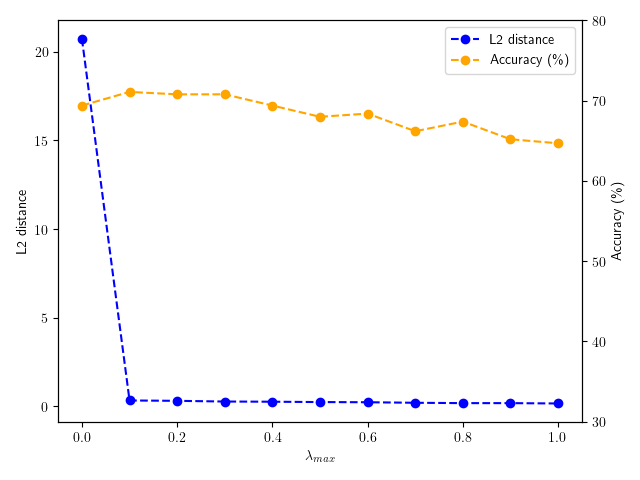
\includegraphics[width=8cm]{figures/analysis.png}
	\end{tabular}
	\vspace{-0.3cm}
	\caption{\textbf{The Plot of Hyperparameter Sensitivity on PACS + Alexnet} The orange line represents the mean accuracy of the four target domains. The blue line denotes the average L2 distance between the mean representation and the feature of each example.}\label{fig:analysis}
\end{figure}

\subsection{Why ResNet-18 Has a Smaller Gain Than Alexnet?}\label{resnet_discussion}
When we compare the performance gains of Alexnet (Table~\ref{tab:pacs}) and ResNet-18 (Table~\ref{tab:pacs_resnet}), we can see the performance gain in ResNet-18 is much smaller than that of Alexnet. It would indicate the redundancy of the proposed method. When we use the better architecture, the corresponding feature extractor would be able to extract discriminative features. \textbf{Those features may be variant in terms of distribution, but they could be considered invariant in terms of performing the task at hand.} Therefore, we need to design algorithms that can learn discriminative representations rather than trying to matching the feature distributions.

